\chapter{Porting TinyOS for Chronos hardware}

This chapter describes the work done, to make TinyOS run on Chronos watch. Firstly, we show how we added a minimal, yet functional, platform to the OS. Then we discuss the methodology used for introducing new code. Afterwards, we go over basic MCU configuration, fundamental for other systems operation. Then we present a conceptual schema of the watch circuits that, most notably, shows connections between its elements. The remainder part of the chapter describes the hardware drivers we have created, starting with MCU internal systems and going outwards towards the peripherals.

\section{Adding a minimal functional platform}

The first milestone of our project, was to get to the point, where we could compile the \emph{Null} application and upload its image to the watch. Although this application is of little use, it does basic system initialization, therefore allowing to verify the build configuration. The additional benefit was that we could learn much about TinyOS build process.

To compile code for MSP430 architecture, we used the \emph{\bf msp430-gcc}. This was an obvious choice, because NesC compiler has built in support for it. Its installation wasn't, however, as easy as one might expect. Namely packages provided in Ubuntu were too old and did not contain headers for \emph{CC430F6137} MCU. In the end we've removed all related system packages and built the \emph{msp430-gcc} from sources, using most recent version available at the time - 4.6.2.  In addition to the compiler, tools like \emph{msp430-gdb} and \emph{mspdebug} were also installed.

The \emph{\bf mspdebug} tool is particularly important for Chronos development, as it allows to flash software on the watch through the USB debug dongle.  Additionally it also allows to debug code running on the watch, by providing a primitive gdb server, to which mentioned \emph{msp430-gdb} is able to connect\footnote{It's imperative to use the most recent version of \emph{msp430-gdb} with \emph{mspdebug}, because older versions are not compatible with it.}.

Afterwards, the {\bf NesC compiler} was installed from sources, rather than packages, followed by the TinyOS distribution. We choose a clean upstream version provided by \cite{TOSnet}. It contained some tools and scripts that also needed to be built and installed.

At this point we had a functional TinyOS installation, capable of targeting MSP430 based boards, like the \emph{telosb}. We choose to name, the new platform for our watch, \emph{chronos}. To make if fully functional, we had to create a few files under \emph{tos/platforms/chronos} path, among which only \emph{.platform} was non-trivial. This configuration file, holds various compilation parameters. In it, we had to specify the exact MCU model used in the watch, so that the generated binary images would have correct offsets for the code segment (0x8000) and the interrupt vector (0xFF80).

We also wanted the build process of an application, to be initiated with a standard TinyOS make command:
\begin{lstlisting}[numbers=none, language=bash]
  $ make chronos install
\end{lstlisting}
For this to work, we had to add a configuration file under \emph{tos/support/make} path. The \emph{chronos.target} file adds our platform to the build system, that in turn takes care of the exact NesC compiler invocations. To make the image automatically install on the device, file \emph{mspdebug.extra} was added under \emph{tos/support/make/msp} path, which invokes the commands that program Chronos.

These changes may seem obvious, but it took quite some time to work them out. Eventually we've reached the point where, the \emph{Null} application was successfully installed on the watch.

\section{Code creation methodology}

The next step, was to add the code that would make the watch operational. Generally it's considered a good programming practice to reuse existing code rather than write it from scratch. Existing code tends to be more tested and can save considerable time, especially when it contains nontrivial constructions, that would otherwise require a test and debug cycle to discover. Moreover such situations are especially frequent when dealing with hardware. Our project was quite time constrained from the beginning and various delays were to be expected further on. In these circumstances saving time wherever possible was particularly important. We benefited greatly, from the fact that TinyOS code licensing is very liberal, allowing for free use, except few very reasonable restrictions like preserving the license headers in files.

Nevertheless not all goals could be completed by adapting existing components. In such cases, where no drivers in NesC were available, we had to fall back to the hardware documentation in the form of datasheets. They describe hardware's behaviour very well, though sometimes, certain issues were only discovered and compensated for, after code was implemented and ran. As a rule, documentation very low lever, describing only control registers available on the device. All higher abstraction layers had to be devised and implemented by the developer. This is a tedious task and applying the Hardware Abstraction Architecture eases it enormously. We didn't know that from the beginning though, so some designs follow it better than others. Besides, in practice boundaries between layers aren't always clear.

Few times we encountered code that was close to what we needed, but some hardware differences made it impossible to use it directly. Modifications had to be done before it could be added to Chronos platform. In these cases we had to mix above approaches, studying the datasheets to understand inner workings of the code. However, we've found that both contributed to better understanding. Code told us much about the inner workings of the hardware and datasheets helped to understand the constructions used in the code. Most notably such approach was used to port the low level radio driver, but the principle extends to other components. As a rule, it was much easier to understand operation of a hardware device if, even a crude, driver implementation was available.

To implement the code, we first used traditional terminal based tools, like the \emph{vim} editor. Later on, when we've discovered the fine \emph{Yetti 2} plugin, we've started using \emph{Eclipse} with all its benefits. This increased our productivity considerably. Also there is no simulator of the watch available. Therefore all testing had to be done by uploading images to the hardware and observing its responses. At first we didn't even know if the programming was successful, but then when LCD display became available followed by the serial console and ultimately visual debugger, the process became quite seamless. See Appendix \ref{ch:prog_env} for details.

Finally, in what we believe is \emph{the way} to create code for mobile platforms, we tried to use \emph{TOSMOCK} for module unit-testing. This technology, however, became available too late to be widely used in our code.

\section{MCU configuration}

The MCU configuration was made much easier, thanks to the existence of a partial port of TinyOS to a similar hardware platform. The Texas Instruments \cite{EM430}, shown in Figure~\ref{fig:em430_board}, is a development board which uses the exact same \emph{CC430F6137} MCU chip as Chronos does. Work on the port was done as a part of the \cite{OSIAN} project. Though the Chronos and the EM430 differ in peripherals, much of the internal MCU configuration code was compatible and we've decided to reuse it.  Minor modification was required, to meet our coding standards and fix a few issues.
\begin{figure}[h]
  \centering
  \includegraphics[width=0.8\textwidth]{img/em430_board.jpg}
  \caption{The Texas Instruments EM430F6137RF900.}
  \label{fig:em430_board}
\end{figure}

All the MCU configuration is done in the \emph{PlatformC} and the \emph{PlatformP} components, shown in Figure~\ref{fig:platformc}.
\begin{figure}[h]
  \centering
  \includegraphics[width=0.9\textwidth]{diagrams/platformc.eps}
  \caption{\emph{PlatformC} performs MCU initialization.}
  \label{fig:platformc}
\end{figure}
The first step that \emph{PlatformP} takes is disabling the watchdog. Otherwise it would shortly reset the device. Disabling it, only requires single register assignment and is done inline. In the future we may wish to use the watchdog to increase Chronos's reliability, but it wasn't a priority in this stage of the project.

One of the primary MCU responsibilities is to provide clocks and timing for other subsystems. First, let's look at the timers. In Section \ref{ch:timer_subsystem} we finished introducing TinyOS timer library, saying that the \emph{HilTimerMilliC} is provided by each platform. Continuing that discussion, Figure~\ref{fig:hil_timer_milli_c} shows a simplified structure of this component, as it is provided by the \emph{chronos} platform.
\begin{figure}[h]
  \centering
  \includegraphics[width=0.9\textwidth]{diagrams/hil_timer_milli_c.eps}
  \caption{Structure of Chronos's \emph{HilTimerMilliC}.}
  \label{fig:hil_timer_milli_c}
\end{figure}
We'll explain it's operation in bottom up order. The \emph{Msp430Timer32khzC} gives access to one of the hardware timers. \emph{Msp430AlarmC} uses it to provide an \emph{Alarm} interface with 32kHz granularity and 16 bit range. Then it is transformed by \emph{TransformAlarmC} into a wider 32 bit alarm with 1ms (actually 1024$\upmu$s) granularity. Finally, this alarm is converted into a timer and virtualized. Note that these transforming components all come from the TinyOS library.

Millisecond granularity isn't, however, sufficient for some of Chronos peripheral drivers. Delays on the order of microseconds are needed, but we didn't want to resort to active waiting. Having latency and memory footprint in mind, we decided to implement virtualized 16 bit microsecond alarms\footnote{Note, that microsecond timing is quite imprecise. Firstly it's difficult to get an event fired after less than 10$\upmu$s and the exact firing time can vary by as much as 25$\upmu$s. Still, if you need to wait 37$\upmu$s, a microsecond alarm is the best choice.} in addition to millisecond timers. They are more light-weight than timers would have been, therefore we can use them more liberally. Alarm structure is shown in Figure~\ref{fig:virutal_alarm_micro_16_c} and it's operation is similar to the timers described above.
\begin{figure}[h]
  \centering
  \includegraphics[width=0.9\textwidth]{diagrams/virutal_alarm_micro_16_c.eps}
  \caption{Structure of \emph{VirtualAlarmMicro16C} generic component.}
  \label{fig:virutal_alarm_micro_16_c}
\end{figure}

The MSP430 specific timer code comes from \emph{tos/chips/msp430/timer} library. But for CC430 MCU's, HPL layer has been overwritten with the \emph{tos/chips/msp430/msp430xv2/timer} components, which we've taken from the EM430 port.

The \emph{Msp430Timer32khzC} and  \emph{Msp430TimerMicroC} components, used above, provide access to 16 bit hardware counters Timer\_A0 and Timer\_A1, running at 32kHz and 1MHz respectively. They are implemented in this new HPL layer, but their structure is relatively simple and mundane so we will omit it. For details, see mentioned libraries.

Now we'll describe the configuration of Chronos clocks, which generate driving signals for timers and other subsystems. There are three major clocks available on the platform. The first is the {\bf REFOSC}, which uses an internal 32kHz oscillator. The second is the {\bf DCO} that uses an internal high frequency digitally-controlled oscillator, which we run at 32MHz. Third the {\bf XT1}, powered by an external 32kHz crystal oscillator. This last one supports very low power operation. MCU can be left in deep sleep state, while the external oscillator drives the clock that can then wake it. In this mode, only a tiny current is consumed. We didn't, however, utilize this option leaving it for future research.

MCU subsystems are actually fed from so called clock sources. This indirection allows to modify the clock signal before passing it on. In particular, it allows to scale down the frequency by a constant factor. There are three clock sources in CC430 MCUs. The {\bf Master Clock (MCLK)} that drives instruction execution, the {\bf Sub-System Master Clock (SMCLK)} that drives MCU peripherals and finally the {\bf Auxiliary Clock (ACLK)} that drives subsystems where slower frequencies are needed.

Clock configuration is done by the \emph{Msp430XV2ClockC} component, which is part of the \emph{tos/chips/msp430/msp430xv2/timer} library. Its structure is presented in Figure~\ref{fig:Msp430XV2ClockC}.
\begin{figure}[h]
  \centering
  \includegraphics[width=1.05\textwidth]{diagrams/Msp430XV2ClockC.eps}
  \caption{The clock configuring component.}
  \label{fig:Msp430XV2ClockC}
\end{figure}
The \emph{Msp430XV2ClockP} module configures all the clocks during its initialization. It does it through the \emph{Msp430XV2ClockControl} interface which is also made available externally, so that applications can tune the configuration if needed. Note that default MCU instruction execution speed can be modified in \emph{Msp430XV2ClockP}. This is possible, through changing the DCO frequency. \emph{Msp430XV2ClockControlP} will set MCLK to half of DCO speed, but it will always set SMCLK to 1MHz\footnote{This is one of the reasons why we drive Chronos MCU at 16MHz rather then maximum 20MHz. It is not possible to scale DCO from 40MHz to 1MHz to drive SMCLK.} and ACLK to 32kHz. Many subsystems depend on these clock sources having constant and known values. In particular, above module, also sets the Timer\_A0 to use the ACLK and Timer\_A1 to use the SMCLK. Moreover USCI uses SMCLK to drive UART, SPI and I$^2$C buses. These settings are summarised in Table \ref{fig:clock_speeds}.
\begin{table}
  \centering
  \begin{tabular}{ | l | l | }
    \hline
    Subsystem & Used frequency \\
    \hline
    DCO & 2MHz, 4MHz, \ldots, 32MHz \\
    REFOSC & 32kHz \\
    MCLK & DCO / 2 \\
    SMCLK & DCO scaled to 1MHz  \\
    ACLK & REFOSC \\
    Timer\_A0 & ACLK \\
    Timer\_A1 & SMCLK \\
    UART, SPI and I$^2$C & SMCLK \\
    \hline
  \end{tabular}
  \caption{Clock frequency convention used in Chronos.}
  \label{fig:clock_speeds}
\end{table}

\begin{lstlisting}
  pmm
    noticed that pmm configuration is necessary after reviewing em430 code
    implementation is custom however and in particular correct
\end{lstlisting}


\section{Overview of the watch's subsystems}

Figure~\ref{fig:}

\begin{figure}[h]
  \centering
  \includegraphics[width=1.05\textwidth]{diagrams/chronos_schema.eps}
  \caption{Overview of Chronos subsystems and circuit board}
  \label{fig:chronos_schema}
\end{figure}


% To enable wrapped line navigation:
% map j gj
% map k gk

% Vim settings:
% vim: set nonumber:
% vim: set linebreak:
% vim: set wrap:
% vim: set textwidth=0:
% vim: set fo+=t:
